\section{Teilversuch 2: Mikroskopieren mit dem Foldscope}
	\label{sec:tv2}
	\begin{tabularx}{\textwidth}{l p{1mm} X}
		\toprule
		\tou{Versuchsziel} && Aufbau des Foldscopes \\
		\tou{Messmethode} && Qualitative Beobachtungen \\
		\bottomrule
	\end{tabularx}
	\vspace{-\baselineskip}
	\subsection{Durchführung}
		Um die Proben für die Untersuchung mit dem Foldscope vorzubereiten wurden die Präparate nach der Anleitung (Siehe Anhang \ref{appdx:anleitung}) Schritt a) vorbereitet. Für die flüssige Proben wurden die Kunststoffobjektträger mit der kleinen Löcher verwendet und die andere Proben die Kunststoffobjektträger mit der rechteckigen Löcher. 

		Die Löcher der Kunststoffobjektträger wurden erst mit Klebeband bzw. der vorliegenden Deckglasaufkleber überklebt (klebrige Seite zum Loch). Die Deckglasaufkleber wurden überall verwendet, wo die Durchsichtigkeit wichtig war, da das Klebeband oft beim Abrollen weiße Linien und Fingerabdrücke sammelt.  

		Die Proben wurden dann auf der klebrigen Öffnung platziert. Das erfolgte entweder mit einer Pinzette (feste Probe) oder einer Kunststoffpipette (flüssige Probe). Ein weiteres Klebeband bzw. Deckglasaufkleber wurde dann überklebt, sodass die Löcher verschlossen waren. 
		\begin{figure}[H]
			\centering
			\begin{subfigure}[b]{0.3\textwidth}
				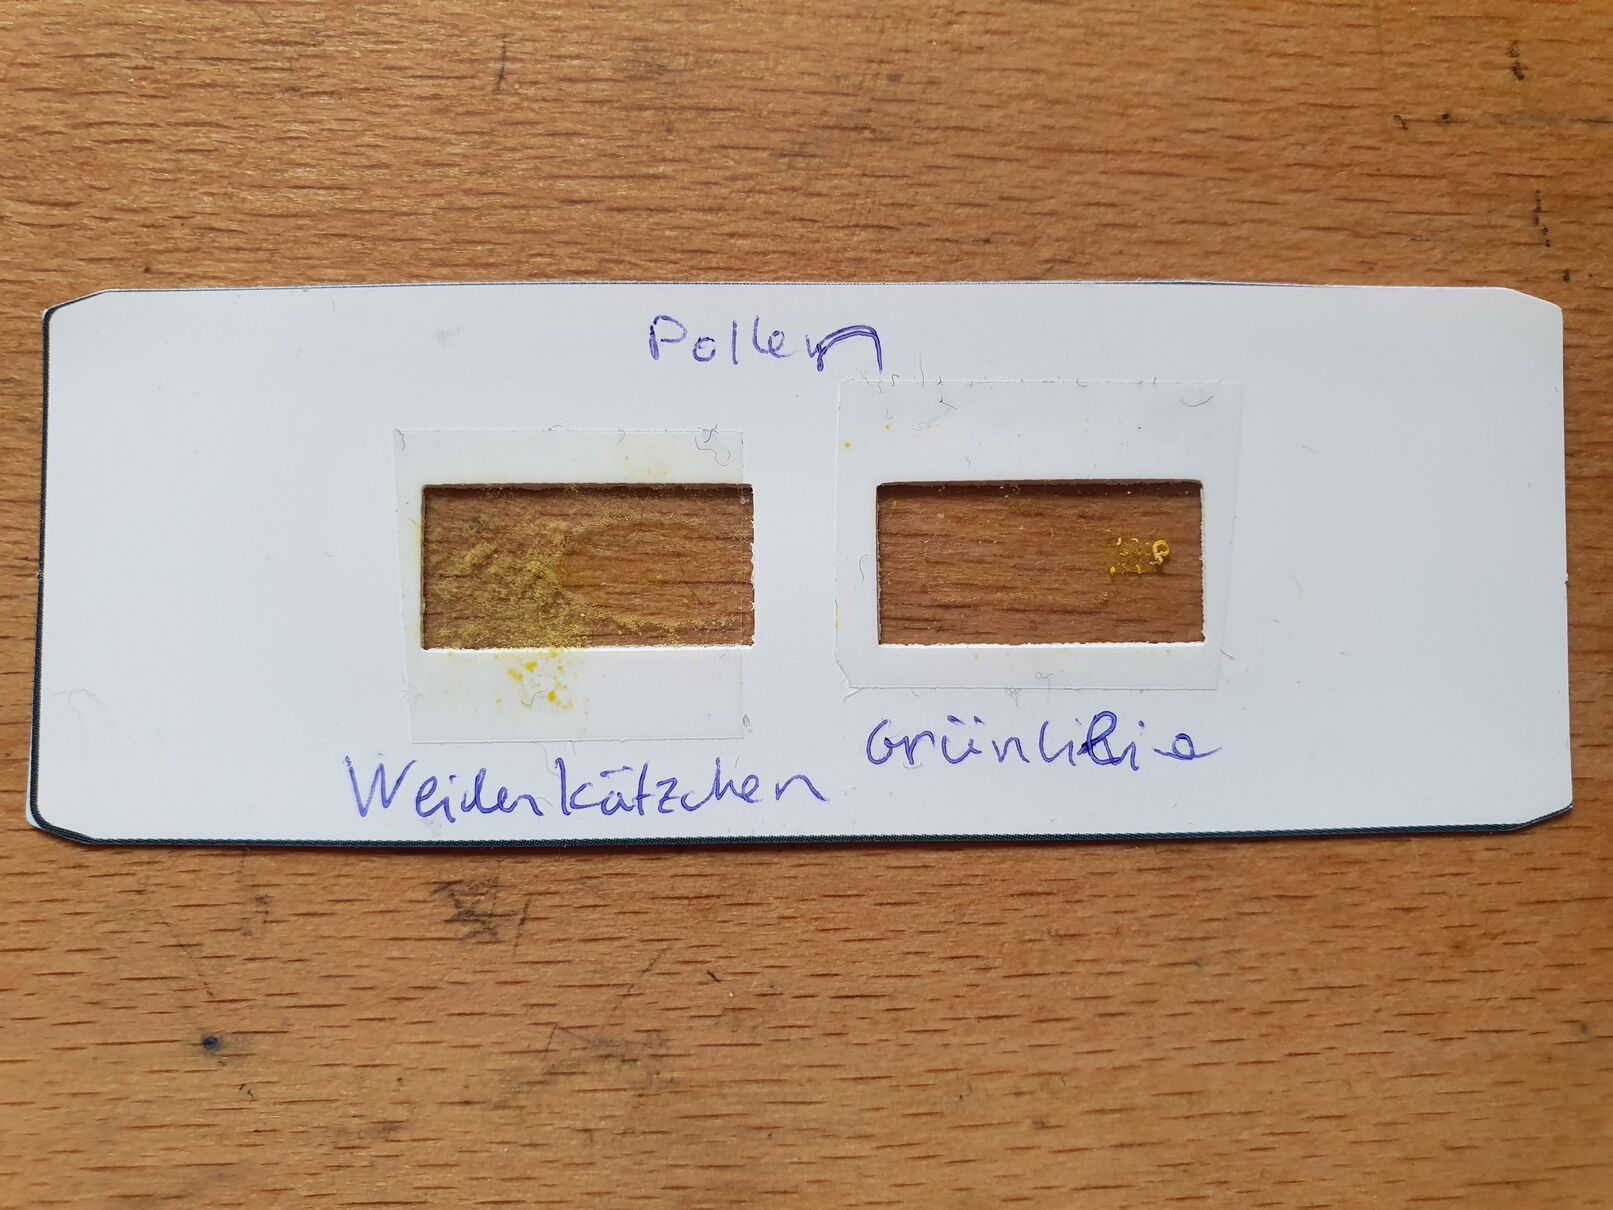
\includegraphics[width=\textwidth]{images/tv2/build-01.jpg}
				\caption{Pollen als Probe}
			\end{subfigure}
			\hspace{5pt}
			\begin{subfigure}[b]{0.3\textwidth}
				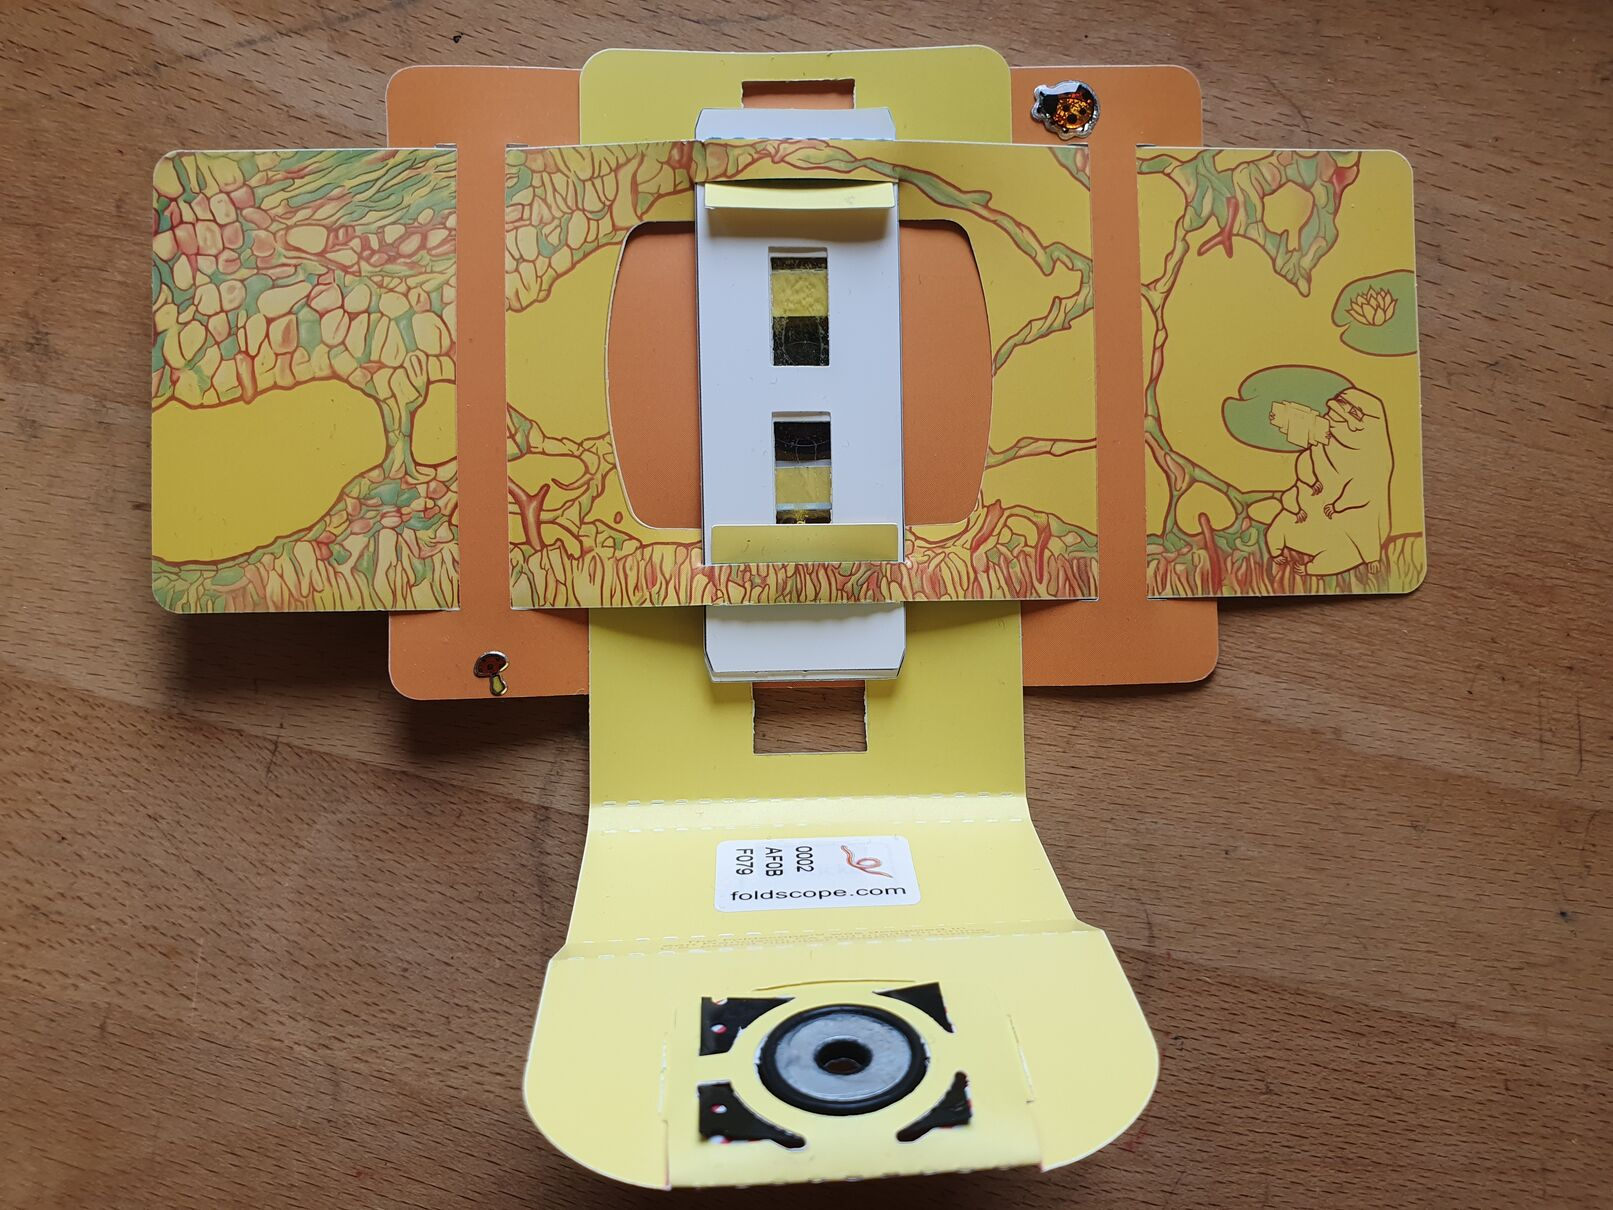
\includegraphics[width=\textwidth]{images/tv2/build-02.jpg}
				\caption{Platzierung im Foldscope}
			\end{subfigure}
			\hspace{5pt}
			\begin{subfigure}[b]{0.3\textwidth}
				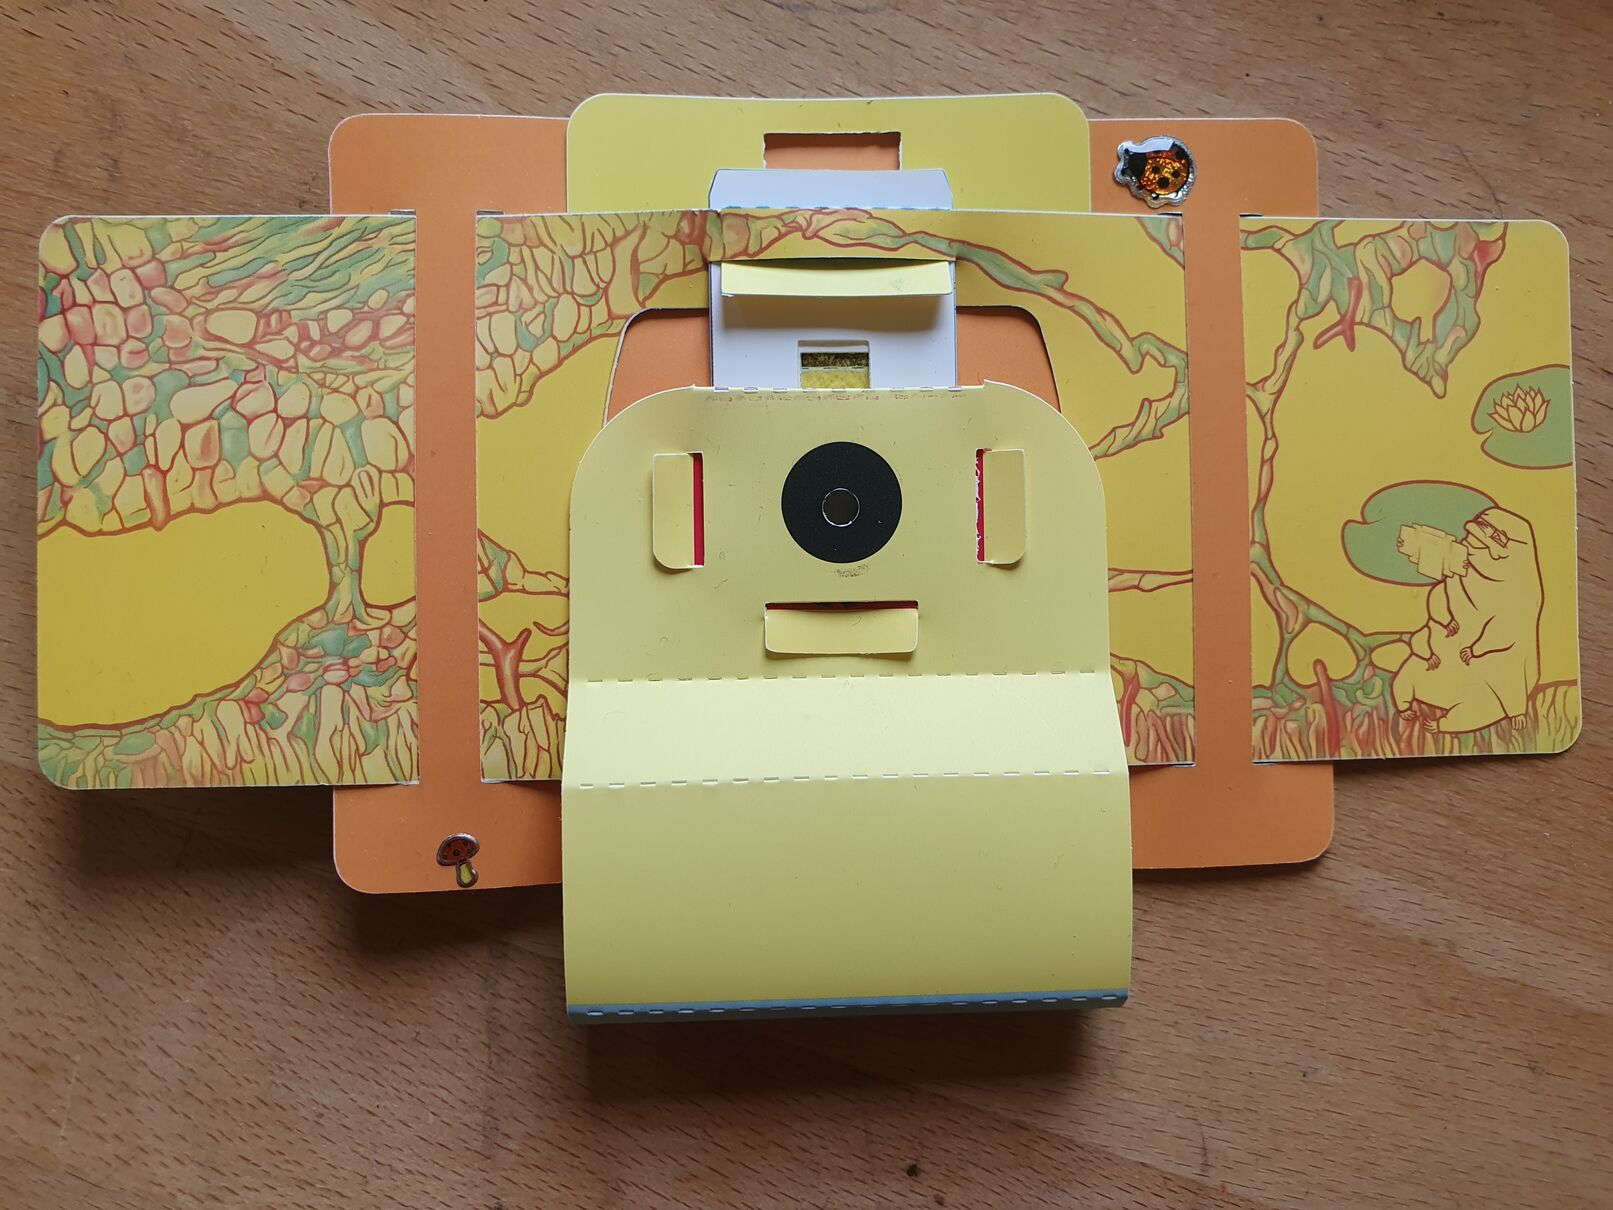
\includegraphics[width=\textwidth]{images/tv2/build-03.jpg}
				\caption{Bereit für die Untersuchung}
			\end{subfigure}
			\caption{Vorbereitung der Präparate für die Untersuchung}
			\vspace{-1em}
		\end{figure}
		Die Präparate wurden dann entsprechend beschriftet, bevor sie in dem Foldscope plaziert wurden. Es wurde auch zwei leere Kunststoffobjektträger hinter dem Präparat (vom Perspektiv des Auges) im Foldscope plaziert, um das Bild besser scharf stellen zu können.

		Nach der qualitative Untersuchung mit der Augen wurden noch zusatzliche Bilder mit dem Smartphone gemacht. Die im Versuch verwendete Smartphones sind:
		\begin{itemize}
			\item OnePlus 2 (ONE A2003)
			\item Samsung Galaxy S10e (SM-G970F)
		\end{itemize}
		Im Fall des Samsung Galaxy S10e wurde nur die 12MP, $f/1.5$-$2.4$, $\SI{26}{\milli\meter}$ Kamera\footnote{\url{https://www.gsmarena.com/samsung\_galaxy\_s10e-9537.php}} verwendet. Die Ultrawide-Kamera wurde wegen Fokusprobleme nicht verwendet. Der dritten Magnetkoppler wurde im beiden Fällen auf der Kamera mit Klebeband geklebt, sodass die Kamera gut mit dem Folscope ausgerichtet ist. 
		\begin{figure}[H]
			\centering
			\begin{subfigure}[b]{0.45\textwidth}
				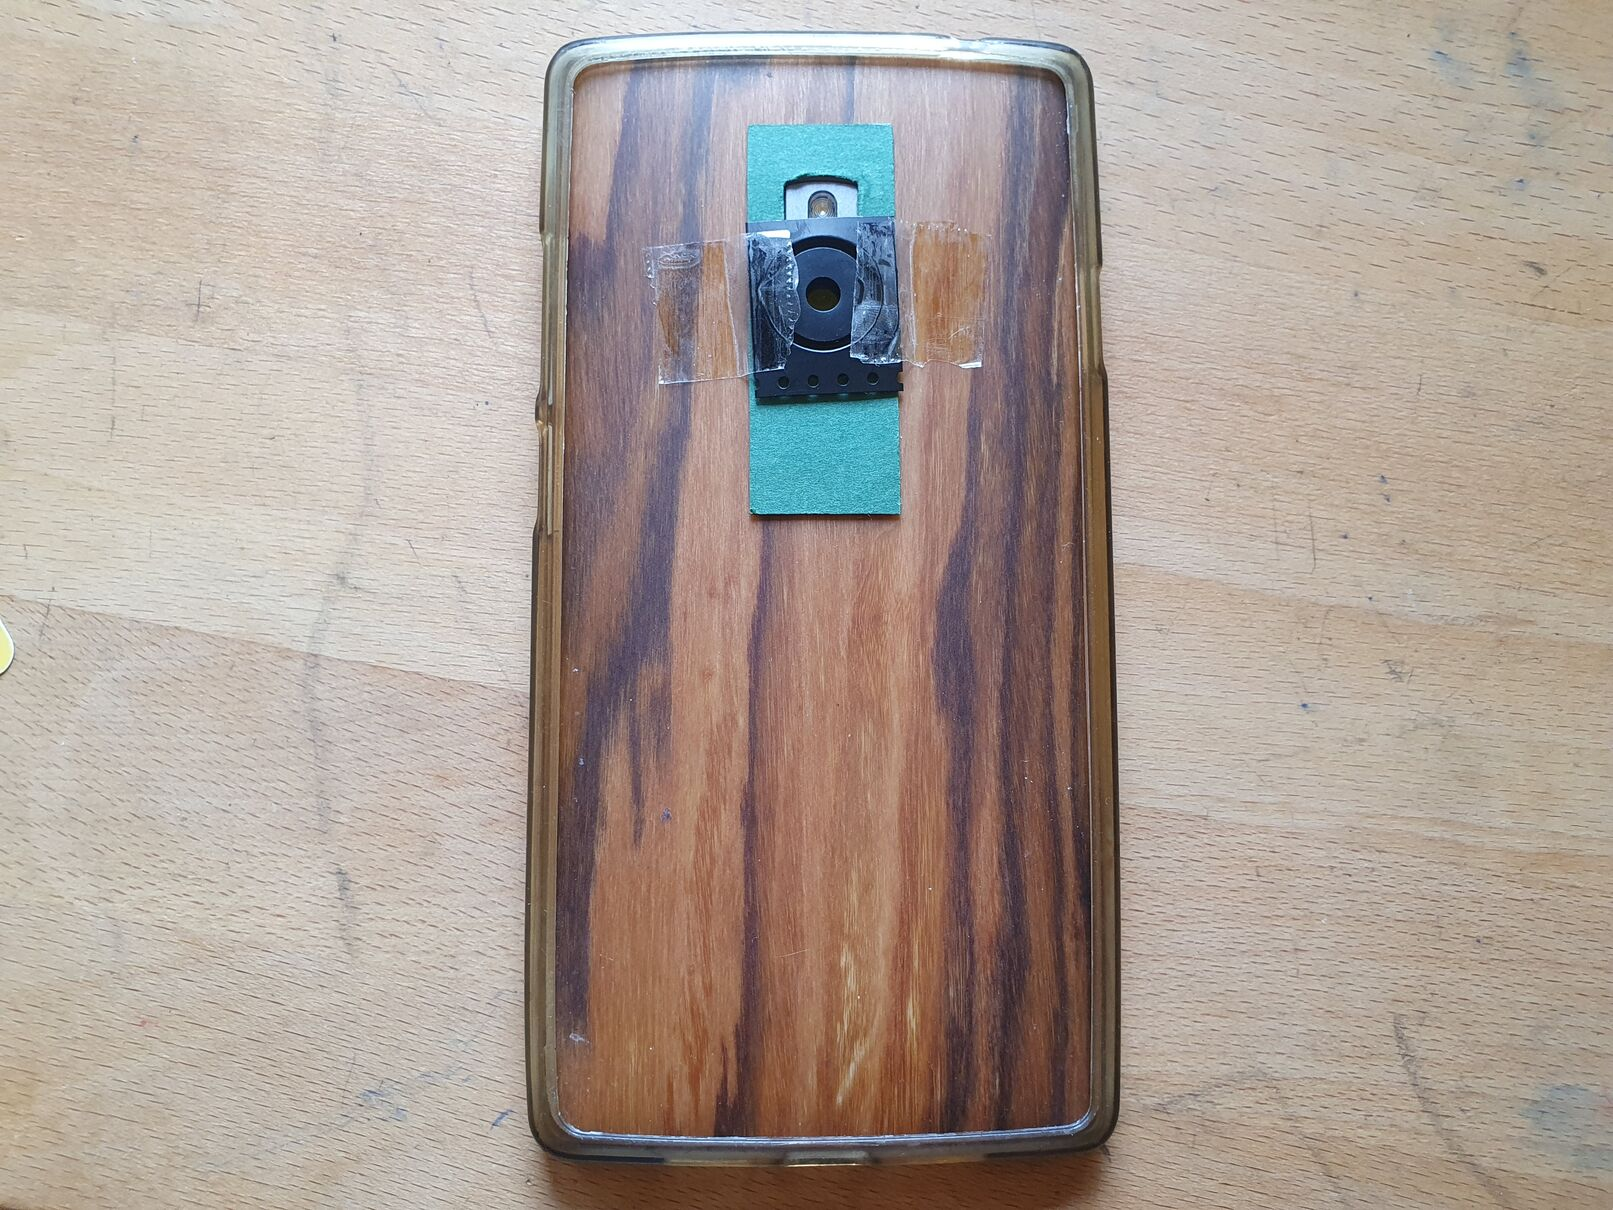
\includegraphics[width=\textwidth]{images/tv2/build-04.jpg}
				\caption{Magnetkoppler auf der Kamera geklebt}
			\end{subfigure}
			\hspace{5pt}
			\begin{subfigure}[b]{0.45\textwidth}
				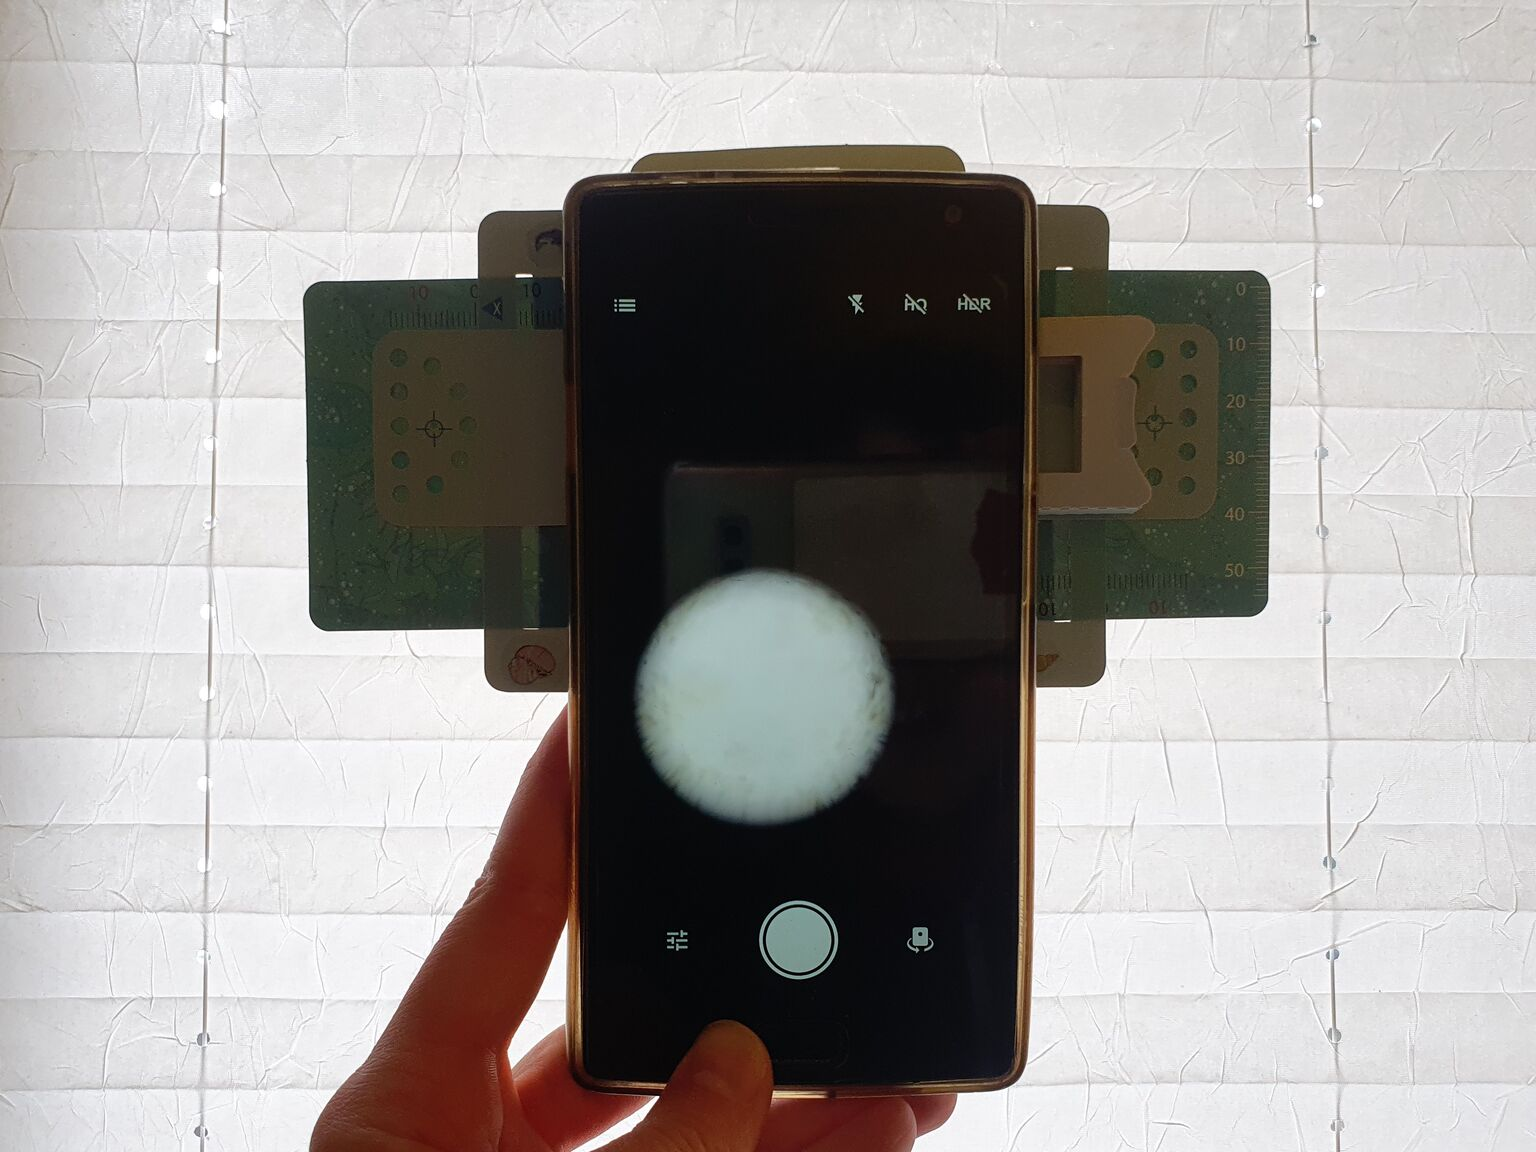
\includegraphics[width=\textwidth]{images/tv2/build-05.jpg}
				\caption{Smartphone gekoppelt mit dem Foldscope}
			\end{subfigure}
			\caption{Fotografieren der Proben mit dem Smartphone}
			\vspace{-1em}
		\end{figure}
		Es ist zu bemerken, dass der Fokusteil der Kamera des Samsung Galaxy S10e nur im Nahfeld funktioniert, wenn der Magnetkoppler aufgeklebt war. 
	\vspace{-1em}
	\subsection{Untersuchte Proben}
		\begin{figure}[H]
			\centering
			\begin{subfigure}[b]{0.3\textwidth}
				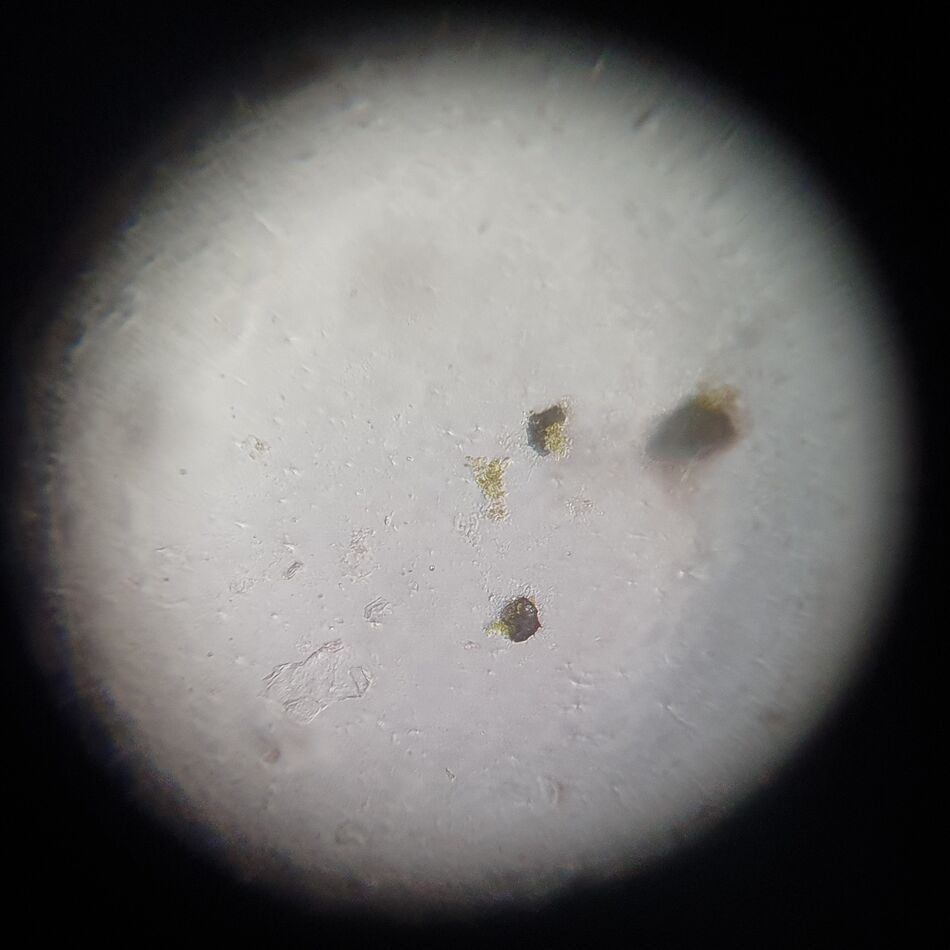
\includegraphics[width=\textwidth]{images/tv2/probe_Aquarium.jpg}
				\caption{Brackwasseraquarium}
				\label{fig:aquarium}
			\end{subfigure}
			\hspace{5pt}
			\begin{subfigure}[b]{0.3\textwidth}
				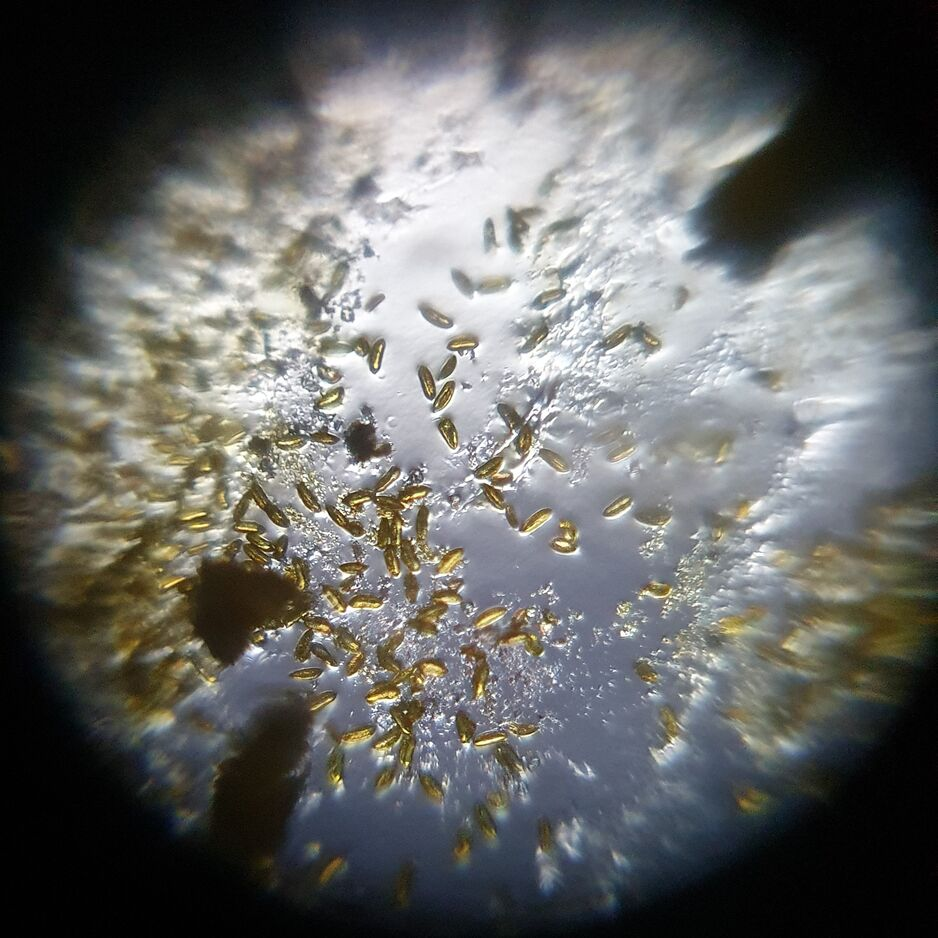
\includegraphics[width=\textwidth]{images/tv2/probe_Gruenlilie.jpg}
				\caption{Pollen aus Grünlilie}
				\label{fig:pollen-g}
			\end{subfigure}
			\hspace{5pt}
			\begin{subfigure}[b]{0.3\textwidth}
				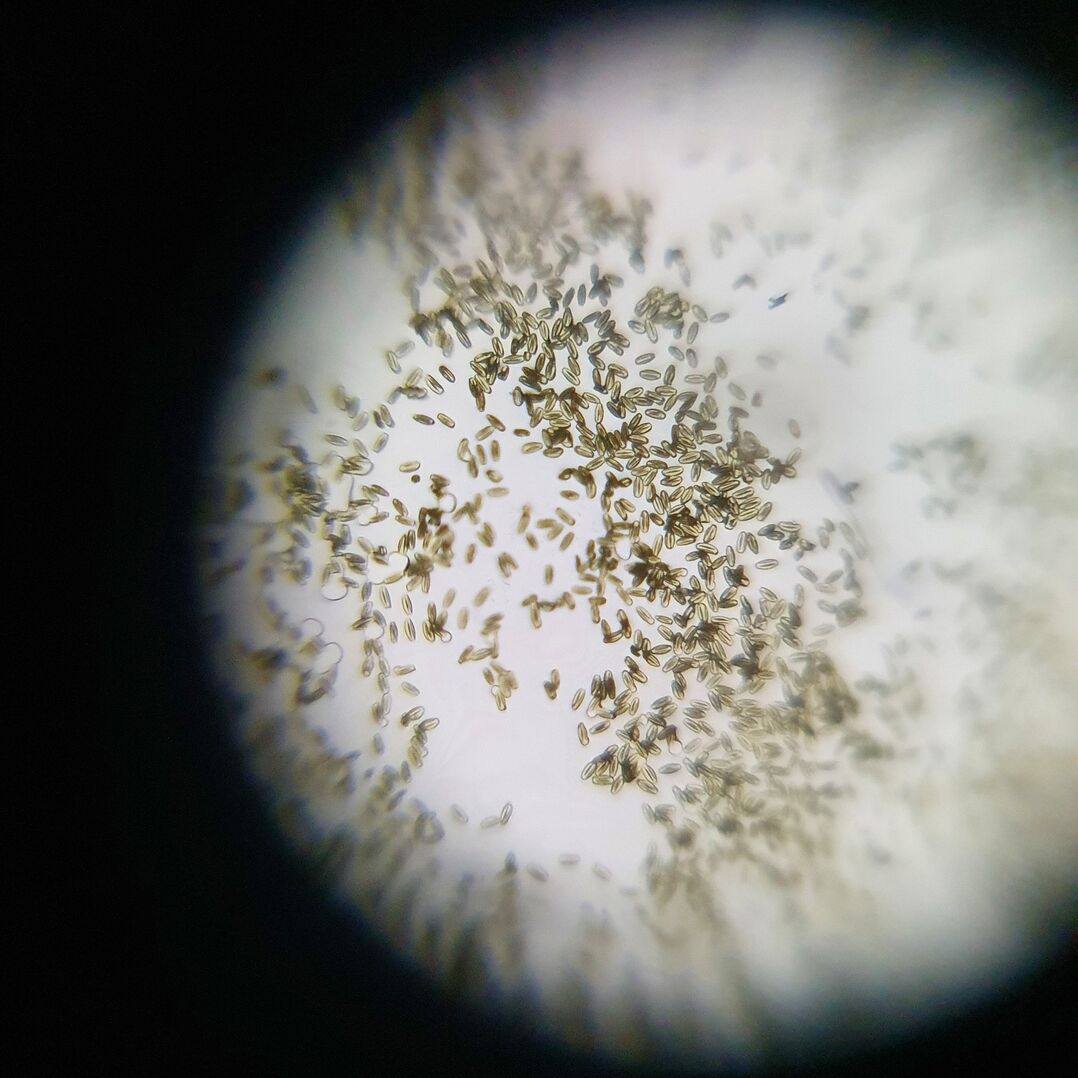
\includegraphics[width=\textwidth]{images/tv2/probe_Weidenpollen.jpg}
				\caption{Pollen aus Weidenkätzchen}
				\label{fig:pollen-w}
			\end{subfigure}
			\\[7pt]
			\begin{subfigure}[b]{0.3\textwidth}
				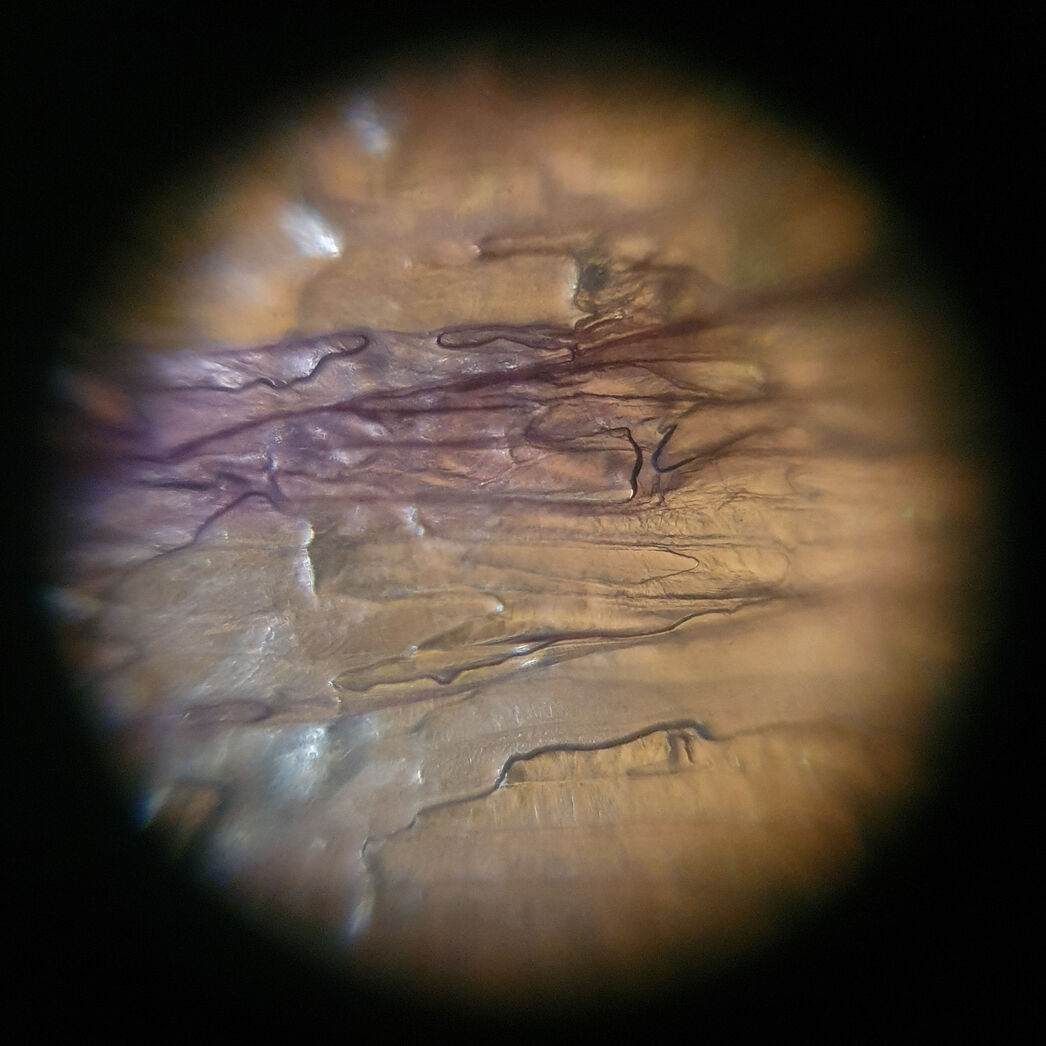
\includegraphics[width=\textwidth]{images/tv2/probe_zwiebel.jpg}
				\caption{Zwiebelhaut}
				\label{fig:onion}
			\end{subfigure}
			\hspace{5pt}
			\begin{subfigure}[b]{0.3\textwidth}
				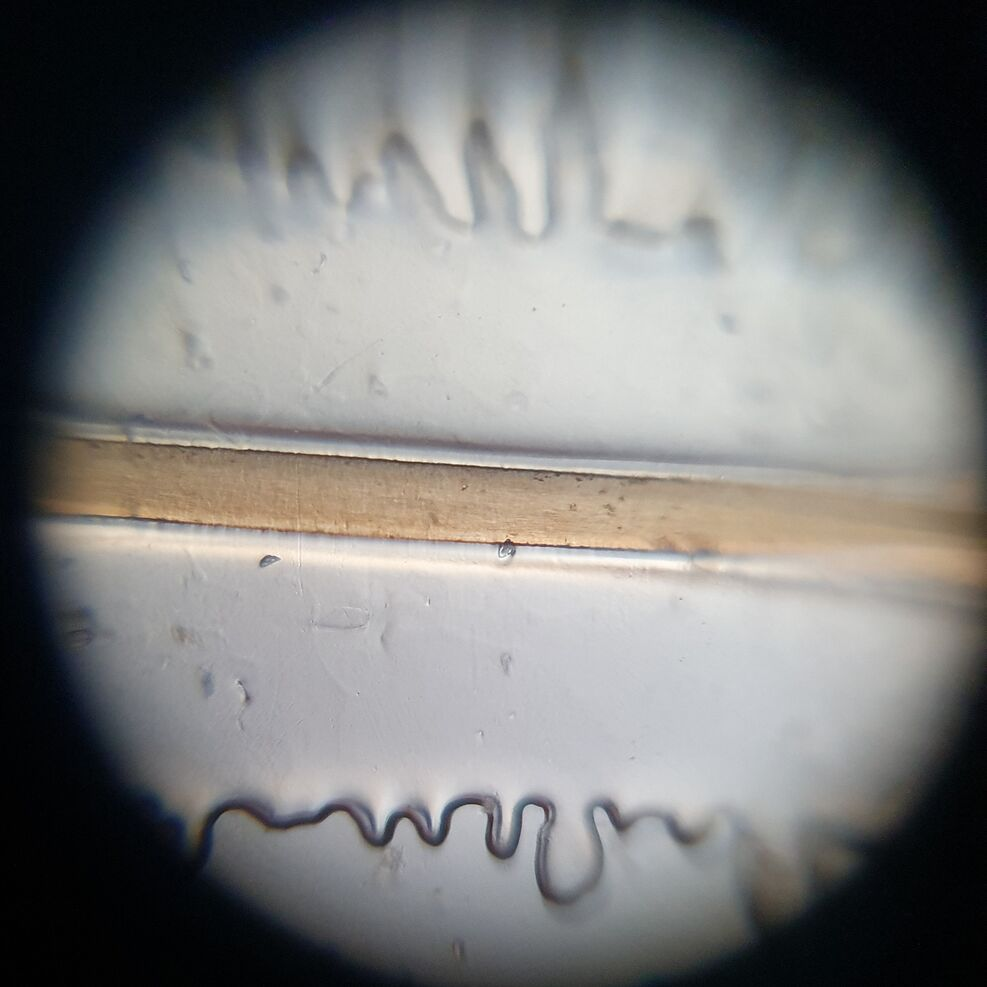
\includegraphics[width=\textwidth]{images/tv2/probe_Haar_Marlene.jpg}
				\caption{Braunes Haar}
				\label{fig:brownhair}
			\end{subfigure}
			\hspace{5pt}
			\begin{subfigure}[b]{0.3\textwidth}
				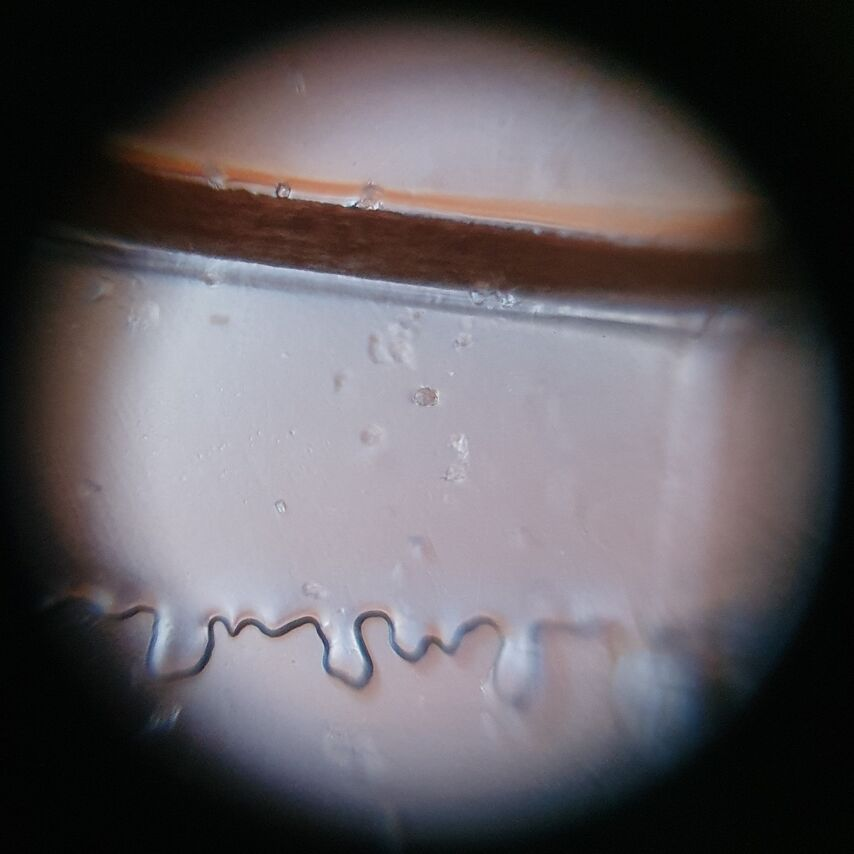
\includegraphics[width=\textwidth]{images/tv2/probe_Haar_Yudong.jpg}
				\caption{Schwarzes Haar}
				\label{fig:blackhair}
			\end{subfigure}
			\caption{Die mit dem Foldscope untersuchten Proben}
			\label{fig:tv2-proben}
			\vspace{-1.4em}
		\end{figure}
		Man sieht hier, dass es stärkere sphärerische Abberationen gibt. Man kriegt infolgedessen nie das ganze Bild im Fokus.
		\begin{center}
			\renewcommand*{\arraystretch}{1.8}
			\begin{tabularx}{\textwidth}{l X}
				Abbildung \ref{fig:aquarium} 
					& Es ist hier grüne Flecken zu sehen, was vermutlich Algen sind. \\
				Abbildung \ref{fig:pollen-g} und \ref{fig:pollen-w} 
					& Die Pollen aus Grünlilie und Weidenkätzchen haben sehr ähnliche Strukturen, was ich nicht erwartet habe. Da das Foldscope eine feste Vergrößerung hat, kann man auch beobachten, dass die Pollen aus Weidenkätzchen ein bisschen kleiner ist als die aus der Grünlilie. \\
				Abbildung \ref{fig:onion} 
					& Wir haben versucht, mit einer verwässerten Lösung von Betaisodona Salbe ($10\%$ Povidon-Iod) die Zwiebelhaut zu färben, aber das war leider nicht erfolgreich. Die Zwiebelhaut bleibt dieselbe Farbe als vor der Färbung. \\[-0.5em]
					& Man sieht hier aber trotzdem Strukturen, die die Zwiebelzellen entspricht.  \\
				Abbildung \ref{fig:brownhair} und \ref{fig:blackhair} 
					& Die Haare sehen strukturell sehr ähnlich aus. In beiden Fällen sind die Haare heller als was man im Alltag wahrnimmt. 
			\end{tabularx}
		\end{center}
		Wir haben im Versuch auch Wasser aus einer Regentonne und verwässerten Joghurt untersucht. Es ist aber im Foldskop nichts zu erkennen. Die Vergrößerung war wahrscheinlich nicht genug, um die Mikroorganismen sichtbar zu machen. 

		Es ist hier auch zu bemerken, dass die Fokussierung besser erfolgt, wenn man zusätzlich zur Steuerung des Fokussteils auch mit dem Finger auf dem Präparat von hinten druckt. Wenn man das Präparat während der Untersuchen verschieben will, soll man mit der Daumen auf der kleinen Löcher der linken und rechten Seite des Linsenhalters das Foldscope halten, bevor man den Linsenhalter und den Probenhalter gegeneinander verschiebt.